%#Split: 01_background  
%#PieceName: p01_background
% p01_background_00.tex
\KLBeginSubjectWithHeaderCommands{01}{2}{研究の位置づけ}{1}{F}{3}{\DCPDVeryFirstPageStyle}{\DCPDDefaultPageStyle}

\section{研究の位置づけ}
%    <<最大 1ページ>>

%s03_background
%begin 背景: 当該分野の状況 ====================
\graysubsection{当該分野の状況: フェイクニュースの自動検出}
SNSの発展で情報を迅速かつ大量に取得・共有が容易になった一方、
悪意により他人を騙すために作られた\textbf{フェイクニュース}も拡散されやすくなった。
特に2020年からCOVID-19の影響による誤情報の拡散であるインフォデミックにより、
メタノール飲用による死亡事故\cite{iraninfo}といった事象が報告された。
以上から騙された人々により社会的損害が起きるため、
\bfundl{フェイクニュース拡散の早期抑制が必要である}\cite{snsinfo}。

フェイクニュース検出へ有識者が調査する\textbf{ファクトチェック}がある。
これは拡散ののち着手されるため、\bfundl{拡散抑制にはならない}。
そのため、自動でフェイクニュースを検出するべく深層学習によって
ファクトチェック結果をラベルとして、記事内容やユーザの反応から教師あり学習で自動検出する研究がある\cite{Wang:2018:EEA:3219819.3219903}。
%end 背景: 当該分野の状況 ====================

%begin 背景: 課題 ====================
\graysubsection{課題}

\setlength\intextsep{0pt}
\setlength\textfloatsep{0pt}
\begin{wrapfigure}{r}[7pt]{0.31\linewidth}
    \vspace{-5mm}
    \centering
    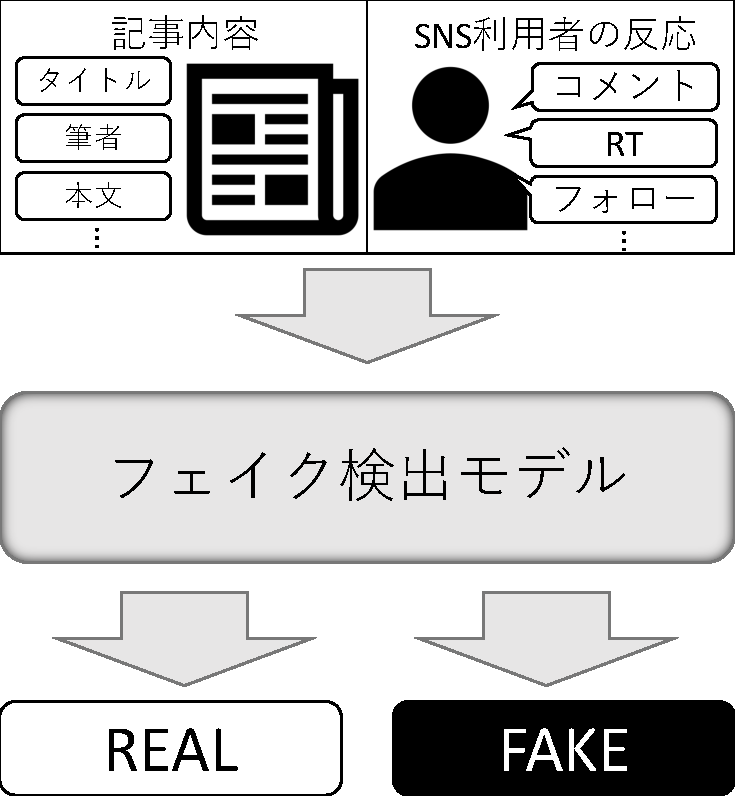
\includegraphics[width=0.31\textwidth]{figs/base_model.pdf}
    \vspace{-1cm} 
    \caption{フェイクニュース自動検出の基本的な流れ}
    \label{fig:objects}
\end{wrapfigure}

フェイクニュース自動検出が抱える課題は以下の通りである。
\begin{description}
    \item[早期検出と正確性の両立] \mbox{}\\
        記事内容に加えてユーザの反応を扱うと検出性能が改善した報告がある\cite{Wu:2018:TFF:3159652.3159677}一方、
        ユーザの反応を十分に得るには時間がかかるため、\bfundl{高い正確性と早期検出を両立できない}。
    \item[日本語データセット不足] \mbox{}\\
        深層学習による実現は、正解ラベルとして多量のファクトチェック結果を要する。
        このファクトチェックが活発な地域差の影響でデータセットが\textbf{英語に集中}\cite{fakenewsnet}している。
        もし\textbf{日本語を対象}とした場合、ファクトチェック結果が不足しているためラベル付きデータセットによる\bfundl{教師あり学習ができない}。
    \item[汎化性能不足] \mbox{}\\
        モデルによって、例え同じニューストピックでもデータセットを変えると分類性能が大幅に劣化する\cite{coviddiff}。
        絶えず変化する社会情勢を鑑みて、\bfundl{汎化性能がないモデルは実際の運用に向かない}。
\end{description}
%end 背景: 課題 ====================

%begin 着想に至った経緯 ====================
\graysubsection{本研究計画の着想に至った経緯}
私は修士過程で\bfundl{英文フェイクニュース早期検出の研究を行った}。
記事に対するユーザのコメントが検出に有用とする先行研究をベースに、
早期検出を想定して\bfundl{少ないコメントから更にコメント内容を自動生成}して検出するモデルを実装した。
実験にてコメントを生成した上で分類することでより多くのフェイクニュース検出を実現した(査読付き海外IEEE学会 発表済\cite{ines})。

一方、国内研究会で発表したところ想定以上に日本語での実現に対する期待を受けた。
日本は英語圏に比べファクトチェックされた記事が少なく、
\bfundl{データセットを作ってモデルを実装するにはラベルが足りない}。
このラベル不足を補う方法として、少量のラベル付き記事と多量のラベルなし記事にユーザの初期反応から
弱いアノテーションを付加して学習を行う弱教師あり学習を行う研究\cite{mwss}に着目した。
日本語で同じ構成のデータセットを作成し、分類を行うモデルを実装することで実現可能と考えた。

%end 着想に至った経緯 ====================

{\footnotesize 
%\vspace{1cm}
\begin{twobibliography}{99}
    \setlength{\parskip}{0cm}
    \setlength{\itemsep}{0cm}
    \bibitem{iraninfo} H H-M, \textit{et al.} \textit{Critical Care} 24.1 2020: 1-3.
    \bibitem{snsinfo} S. Tasnim, \textit{et al.} \textit{JPMPH} 53.3 2020: 171-174.
    \bibitem{Wang:2018:EEA:3219819.3219903} Yaqing W, \textit{et al.} {KDD'18}, pp. 849-857. 2018.
    \bibitem{Wu:2018:TFF:3159652.3159677} Liang W \& Huan L. \textit{WSDM '18},  pp. 637-645, 2018.
    \bibitem{fakenewsnet} Kai S,\textit{et al.} \textit{Big Data 8.3} 2020: 171-188.
    \bibitem{coviddiff} Yejin B, \textit{et al.} \textit{arXiv preprint arXiv:2101.03841} 2021.
    \bibitem{ines} Yuta Y, \textit{et al.} \textit{INES}. 2020.
    \bibitem{mwss} Kai S, \textit{et al.}  \textit{arXiv preprint arXiv:2004.01732} 2020.
\end{twobibliography}
}
% p01_background_01.tex
\KLEndSubject{F}


